
\RequirePackage{algorithmic}


\documentclass{beamer}

\usepackage[utf8x]{inputenc}
\usepackage{default}
\usepackage{ beamerthemesplit}



\title{Robot Localization Simulator}
\author{ Prateek Garg, Kumar Ashwani, Apurv Verma }
\date {\today}

\begin{document}
\frame{\titlepage}

\frame
{
  \frametitle{Acknowledgement}
We would like to acknowledege Assistant Professor Apurva Mudgal for helping us understand the difficult Robot Localization Algorithm.
 His supervision made it appear all very easy.
 We are also thankful to the ever enthusiastic CGAL community for helping us with the various CGAL issues.


}

\frame
{
  \frametitle{Introduction}

A robot is placed at an unknown point inside a simple polygon $ P $. The robot has a map of 
$ P$ and can compute visibility polygon from its current location. The robot must determine its correct 
location inside the polygon $P $ at a minimum cost of travel distance.

}


\frame[allowframebreaks]
{
  \frametitle{Robot Localization Algorithm}


{\bf Input:}\\
Map polygon $P$, the visibility polygon $V$.
\\
{\bf Output:}\\
The robot localizes to its actual position $h \in H$
\\
\begin{algorithmic}[1]
  \STATE Compute the set of hypotheses $H$.
 \WHILE{ $ | H | > 1$ } 
  \STATE Compute the majority-rule map $P_{maj}$
  \STATE Compute the polygons $G_{ij}$ for each pair of hypotheses, $h_{i}$ and $h_{j}$
  \STATE Compute the majority rule map $K_{i}$ of $G_{ij}$'s
  \STATE Find the edges on the boundary of $K_{i}$ which are not on the boundary of $P_{maj}$
  \STATE Draw grids and compute the set of coordinates $Q_{H}$ on these edges.
  \STATE Make instance $I_{P,H}$  of $\frac{1}{2}$ -Group Steiner Problem
  \STATE Solve $I_{P,H}$ to compute a half computing path $C \subset P_{maj}$
  \STATE Half-Localize by tracing $C $ and making observations at coordinates $Q_{H}$
  \STATE Move back to the starting location.
 \ENDWHILE
\end{algorithmic}
}

\frame
{
  \frametitle{Geometrical Algorithms}

Visibility polygon is an indispensable component in the hypothesis generation step of the algorithm. Since CGAL had no inbuilt support
 for computing visibility polygons we implemented the following two routines for our purposes.
\begin{itemize}
 \item Visibility Polygon of a point inside a polygon
 \item Visibility Polygon of an edge of the polygon.
\end{itemize}

}

\frame[allowframebreaks]
{
\frametitle{Visibility Polygon of a Point Inside a Polygon}
\begin{definition}
 {\bf Visibility Polygon of Point:} $p$ is the bounded polygonal region of all points of the polygon visible from $p$.  
\end{definition}

}

\frame
{

{\bf Algorithm}
\frametitle{Algorithm}

\begin{enumerate}
 \item 
Collect all the vertices of the polygon which are visible from the point $P$.
\item
Iterate over the list of visible vertices and for each reflex vertex, compute the spurious vertex introduced in the visibility polygon.
\item
Finally sort all the vertices in an order so that they form a simple polygon.
\end{enumerate}

}

\frame[allowframebreaks]
{
\frametitle{Examples}

\begin{figure}[h]
\begin{center}
\scalebox{0.30}{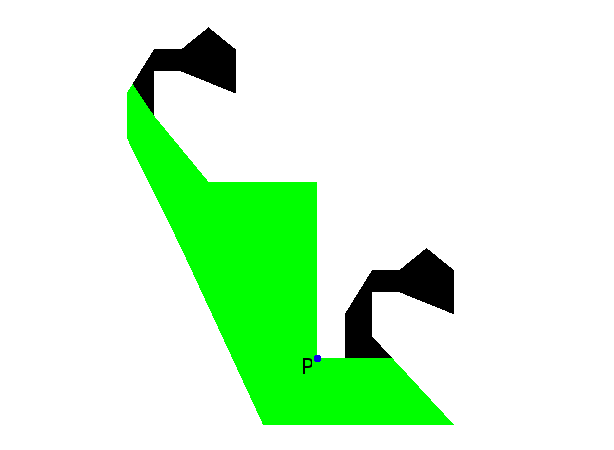
\includegraphics{Images/VisibilityPolygonBird.png}}
\caption{\label{fig:Visibility Polygon of Point}Visibility Polygon of Point}
\end{center}
\end{figure}


\begin{figure}[h]
\begin{center}
\scalebox{0.40}{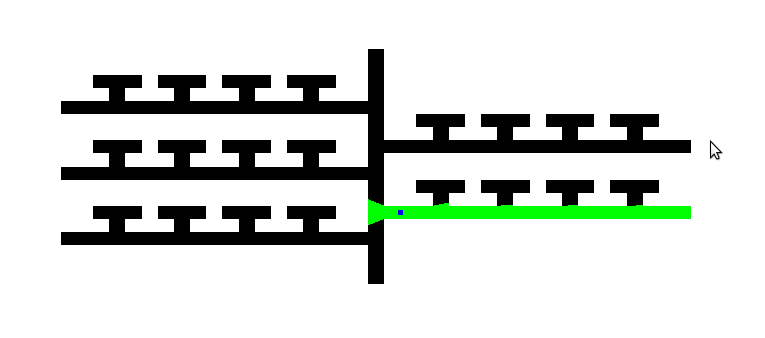
\includegraphics{Images/VisibilityPointOffice.png}}
\caption{\label{fig:Visibility Polygon of Point}Visibility Polygon of Point}
\end{center}
\end{figure}

}

\frame
{
\frametitle{Visibility Polygon of an edge of the polygon}

\begin{definition}
 {\bf Visibility Polygon of Edge:} $e$ is the bounded polygonal region of all points of the polygon visible from any point on the edge $e$. 
\end{definition}

The algorithm for the visibility polygon of an edge has been taken from \cite{key3}.
}

\frame
{
\frametitle{Visibility Polygon of an edge of the polygon}
\begin{figure}[h]
\begin{center}
\scalebox{0.30}{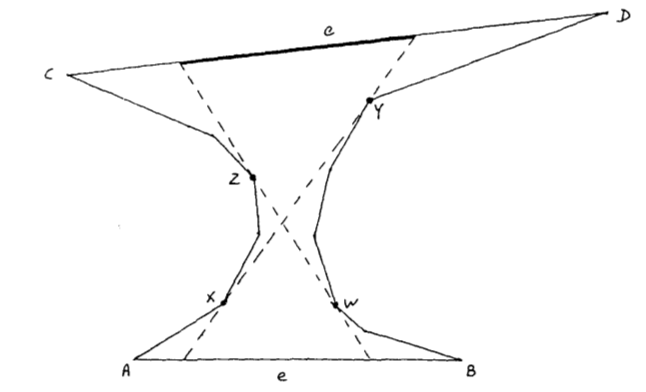
\includegraphics{Images/Cusp.png}}
\caption{\label{fig:Visibility Polygon of Edge}Visibility Polygon of Edge, Illustration taken from:\cite{key3}}
\end{center}
\end{figure}

}

\frame[allowframebreaks]
{
\frametitle{Algorithm}
\begin{enumerate}
\item
Compute the shortest path $P_{AC}$, from A to C and the shortest path $P_{BD}$, from B to D. Call this pair 1.
\item
Similarly compute the shortest path  $P_{AD}$, from A to D and the shortest path  $P_{BC}$,  from B to C. Call this pair 2.
\item
Find out which of these pairs is outward convex. An outward convex pair implies an hourglass shape is formed by the two paths.
\item
If none of the pairs is outward convex this means that no portion of edge $CD$ is visible from any point on edge $AB$ and we can 
completely ignore such an edge.
\item
If one of the pairs is outward convex then without loss of generality, let pair 1 be the outward convex pair. Now compute the shortest 
paths  $P_{AD}$ and  $P_{BC}$.
\item
Let $X$ be the point where path $P_{AD}$ and $P_{AC}$ split and let  $W$ be the point where path $P_{BD}$ and $P_{BC}$ split. Let $Y$ be
the next point on the path  $P_{AD}$ and $Z$ be the next point on the path   $P_{BC}$. Extending $XY$ we get one extreme point of the 
portion of $CD$ visible from $AB$. We repeat this on other side to get the other extreme point.


\end{enumerate}

}

\frame[allowframebreaks]
{
\frametitle{Shortest Path Calculation}
For the calculation of shortest path between any two vertices of the polygon the following property was exploited.
\begin{itemize}
 \item The shortest path must turn only at vertices of the polygon.
 \item It is possible to move from one vertex to the another only if they are visible to each other.
\end{itemize}
}

\frame[allowframebreaks]
{
\frametitle{Visibility Graph}
\begin{definition}
{\bf Visibility Graph}The visibility graph of a polygon can be formed as follows. Draw a vertex corresponding to each vertex in the 
polygon. Draw an edge between two vertices if the line joining the corresponding vertices in the polygon lies completely inside the 
polygon.
\end{definition}


\begin{figure}
\begin{center}
\scalebox{0.4}{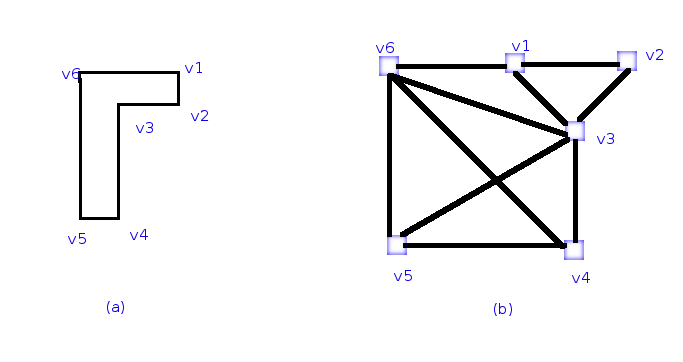
\includegraphics{Images/visibilitygraph.png}}
\caption{\label{fig:Construction} Visibility Graph}
\end{center}
\end{figure}
}

\frame
{
\frametitle{Examples}

\begin{figure}
\begin{center}
\scalebox{0.30}{
\includegraphics{Images/VisibilityLine1.png}}
\caption{\label{fig:Visibility Polygon of Edge}Visibility Polygon of Edge}
\end{center}
\end{figure}

}

\frame
{
\frametitle{Examples}
\begin{figure}
\begin{center}
\scalebox{0.30}{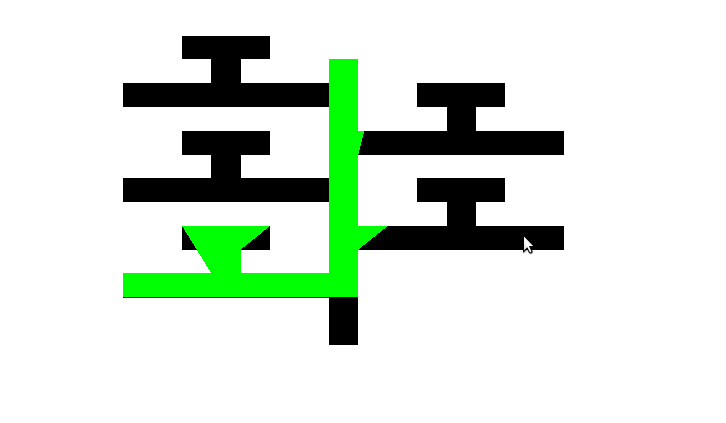
\includegraphics{Images/VisibilityLine2.png}}
\caption{\label{fig:Visibility Polygon of Edge}Visibility Polygon of Edge}
\end{center}
\end{figure}

}




\frame[allowframebreaks]
{
  \frametitle{Robot Localization Algorithm}


{\bf Input:}\\
Map polygon $P$, the visibility polygon $V$.
\\
{\bf Output:}\\
The robot localizes to its actual position $h \in H$
\\
\begin{algorithmic}[1]
  \STATE {\bf Compute the set of hypotheses $H$. }
 \WHILE{ $ | H | > 1$ } 
  \STATE Compute the majority-rule map $P_{maj}$
  \STATE Compute the polygons $G_{ij}$ for each pair of hypotheses, $h_{i}$ and $h_{j}$
  \STATE Compute the majority rule map $K_{i}$ of $G_{ij}$'s
  \STATE Find the edges on the boundary of $K_{i}$ which are not on the boundary of $P_{maj}$
  \STATE Draw grids and compute the set of coordinates $Q_{H}$ on these edges.
  \STATE Make instance $I_{P,H}$  of $\frac{1}{2}$ -Group Steiner Problem
  \STATE Solve $I_{P,H}$ to compute a half computing path $C \subset P_{maj}$
  \STATE Half-Localize by tracing $C $ and making observations at coordinates $Q_{H}$
  \STATE Move back to the starting location.
 \ENDWHILE
\end{algorithmic}
}


\frame
{
 \frametitle{Hypothesis Generation}

\begin{theorem}
 A point, $P$ inside a simple polygon sees atleast one edge of the polygon completely.
\end{theorem}

\begin{definition}
 {\bf Spurious Edge:} In the visibility polygon of a point, an edge is called a spurious edge if it is obtained by extending the line
 joining the point $P$ and a reflex vertex till it meets the polygon.
\end{definition}


\begin{theorem}
 The visibility polygon of a point $P$ has atleast one edge which completely overlaps with an edge of the original polygon.
\end{theorem}

}


\frame
{
\frametitle{Algorithm}
\begin{enumerate}
 \item Iterate over the edges of the polygon and the edges of the map. and find an edge in the map which has the same length and
 orientation as an edge in the polygon.

 \item
 Translate the visibility polygon such that the matching edge of the map polygon
and the visibility polygon coincide.

 \item
 For each of the remaining edges of the visibility polygon, check whether a 
complete match exists or not. If all the remaining edges match, the point where the
origin was translated is added to the set of hypotheses.

\end{enumerate}

}

\frame[allowframebreaks]
{
\frametitle{Examples}

\begin{figure}
\begin{center}
\scalebox{0.40}{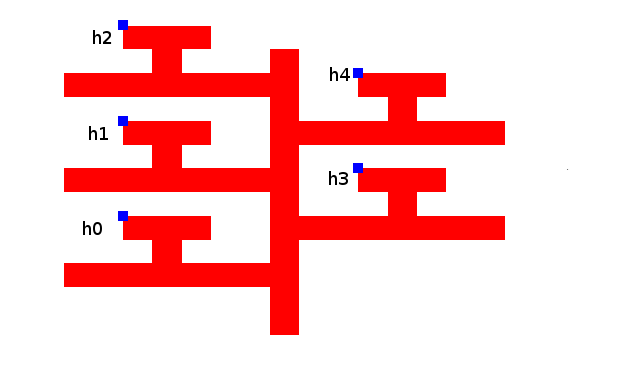
\includegraphics{Images/Hypothesis_office.png}}
\caption{\label{fig:Hypothesis Generation}Hypothesis Generation}
\end{center}
\end{figure}


\begin{figure}
\begin{center}
\scalebox{0.40}{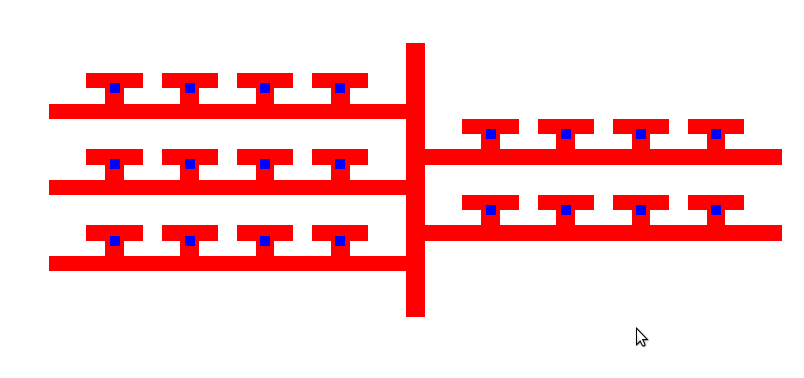
\includegraphics{Images/HypothesisOfficeAnti.png}}
\caption{\label{fig:Hypothesis Generation}Hypothesis Generation}
\end{center}
\end{figure}

}





\frame[allowframebreaks]
{
  \frametitle{Robot Localization Algorithm}


{\bf Input:}\\
Map polygon $P$, the visibility polygon $V$.
\\
{\bf Output:}\\
The robot localizes to its actual position $h \in H$
\\
\begin{algorithmic}[1]
  \STATE Compute the set of hypotheses $H$.
 \WHILE{ $ | H | > 1$ } 
  \STATE {\bf Compute the majority-rule map $P_{maj}$ }
  \STATE Compute the polygons $G_{ij}$ for each pair of hypotheses, $h_{i}$ and $h_{j}$
  \STATE Compute the majority rule map $K_{i}$ of $G_{ij}$'s
  \STATE Find the edges on the boundary of $K_{i}$ which are not on the boundary of $P_{maj}$
  \STATE Draw grids and compute the set of coordinates $Q_{H}$ on these edges.
  \STATE Make instance $I_{P,H}$  of $\frac{1}{2}$ -Group Steiner Problem
  \STATE Solve $I_{P,H}$ to compute a half computing path $C \subset P_{maj}$
  \STATE Half-Localize by tracing $C $ and making observations at coordinates $Q_{H}$
  \STATE Move back to the starting location.
 \ENDWHILE
\end{algorithmic}
}


\frame
{
\frametitle{Majority Rule Map}

The following example taken from \cite{key1} demonstrates the construction of a majority rule map.

\begin{figure}[h]
\begin{center}
\scalebox{0.30}{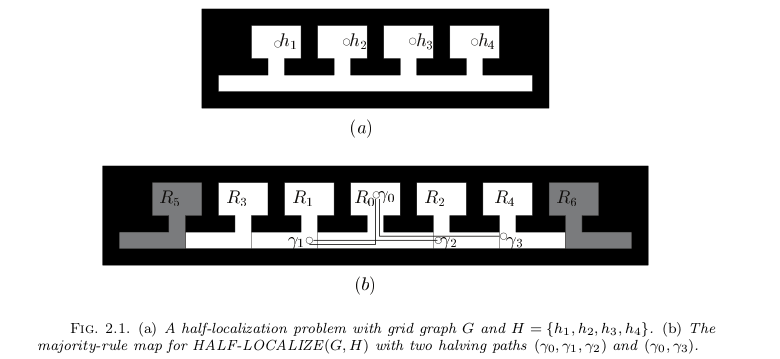
\includegraphics{Images/MajorityMapExample.png}}
\caption{\label{fig:Construction}Majority Rule Map Construction}
\end{center}
\end{figure}
}

\frame
{
\frametitle{Majority Rule Map}

${h_{1},h_{2},h_{3},h_{4}}$ form the set of hypotheses. 
%\vspace{0.1in}
Arbitrarily we choose $h_{1}$ as the origin \vspace{0.1in}.

Next we translate all the remaining hypotheses to $h_{1}$ to obtain the overlay arrangement. The overlay arrangement contains the following faces
$R_{0},R_{1},R_{2},R_{3},R_{4},R_{5},R_{6}$. Recall from the definition of $Maj(\gamma)$

\vspace{0.1in}
$  Maj(R_{0})  =  {h_{1}, h_{2}, h_{3}, h_{4}} $ , $  Maj(R_{1})  =  { h_{2}, h_{3}, h_{4}} $, $ Maj(R_{2})  =  {h_{1}, h_{2}, h_{3}} $,
$  Maj(R_{3})  =  {h_{3}, h_{4}} $ and $  Maj(R_{4})  =  {h_{1}, h_{2}} $ \\
\vspace{0.1in}

In the majority rule map the region $R_{5}$ and $R_{6}$ are blocked because less than half the hypothesis said that they were
 traversable. They have been shown in gray.
}

\frame
{
\frametitle{Algorithm}
\begin{enumerate}
\item
The overlay arrangement can be easily constructed using CGAL's inbuilt Arrangement class. Obtain the translates of the polygon by 
choosing one hypothesis as the origin and shifting other hypothesis to it.
\item
Insert all these translates in CGAL's inbuilt arrangement to obtain all the faces in the overlay arrangement.
\item
Faces which belong to atleast half the hypothesis are marked as part of the majority rule map.
\end{enumerate}

}

\frame[allowframebreaks]
{
\frametitle{Examples}

\begin{figure}
\begin{center}
\scalebox{0.30}{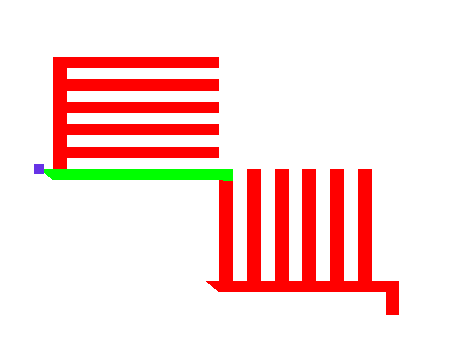
\includegraphics{Images/Scenario4.png}}
\caption{\label{fig:Majority Rule Map}Map Polygon with robot position and Visibility Polygon}
\end{center}
\end{figure}

\begin{figure}
\begin{center}
\scalebox{0.30}{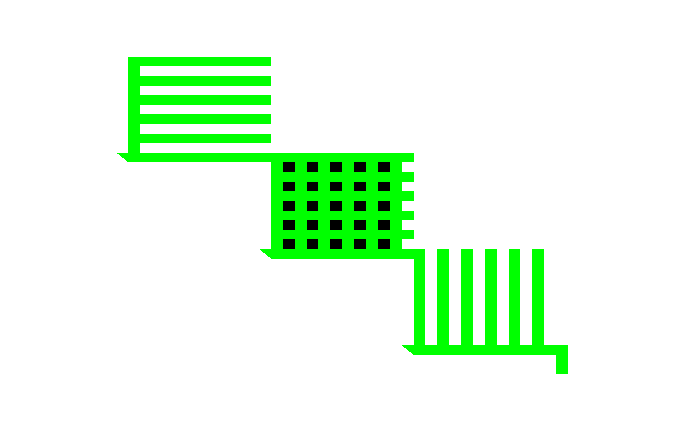
\includegraphics{Images/MajorityMapScenario4.png}}
\caption{\label{fig:Majority Rule Map}Majority Rule Map}
\end{center}
\end{figure}

}


\frame
{
\frametitle{Connected Component containing Origin in $P_{maj}$}
We need to calculate connected component containing origin in $P_{maj}$ as the robot can only move in this area \vspace{0.2in}. 

{\bf Dual graph} of a given planar graph $G$ is a graph which has a vertex corresponding to each face of $G$ and an edge joining two neighbouring faces for each edge in $G$.We also have
a vertex for the unbounded face which is connected to all the faces sharing boundary with unbounded face.  

}
  
\frame 
{
\frametitle{Dual Graph}

\begin{figure}[h]
\begin{center}
\scalebox{0.30}{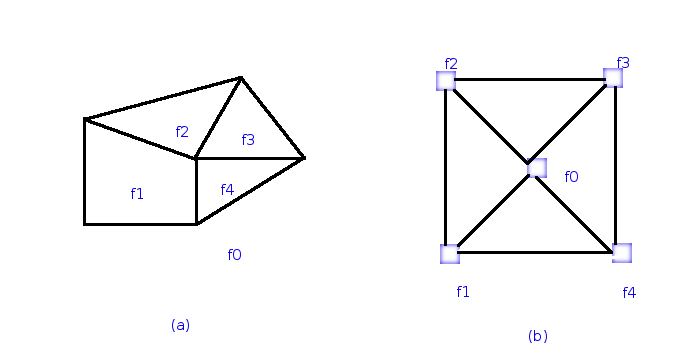
\includegraphics{Images/dualg.png}}
\caption{\label{fig:Dual Graph} (a) Graph $G$ (b) Dual Graph for $G$}
\end{center}
\end{figure}

}

\frame
{
\frametitle{Algorithm for Majority Map}

\begin{enumerate}
 \item Prepare a dual graph $G$ of the traversible faces in the $P_{maj}$.
 \item Find the vertex($v_0$) corresponding to the face containing origin in dual graph G.
 \item Perform Depth First Search [\cite{BOOST}] from $v_0$ to obtain all the connected vertices.
 \item Output the union of the faces corresponding to the connected vertices obtained above.  
\end{enumerate}

}

\frame[allowframebreaks]
{
\frametitle{Examples}

\begin{figure}
\begin{center}
\scalebox{0.30}{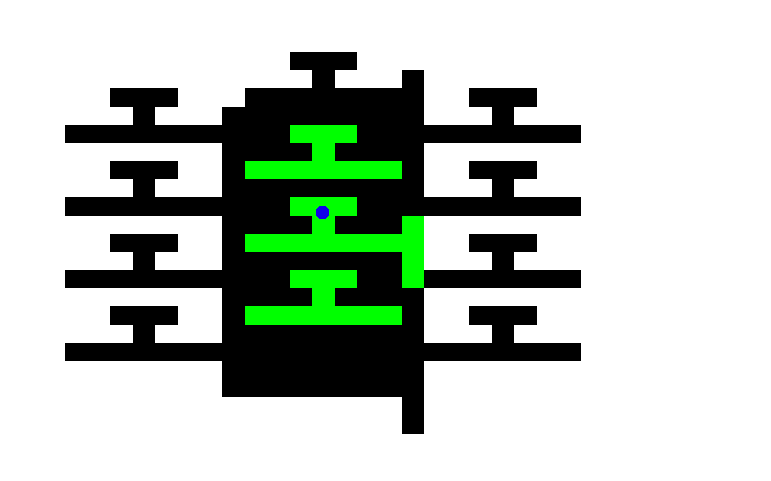
\includegraphics{Images/MajorityMapOffice.png}}
\caption{\label{fig:Connected component} A Majority Map(blue point represents origin)}
\end{center}
\end{figure}

\begin{figure}
\begin{center}
\scalebox{0.30}{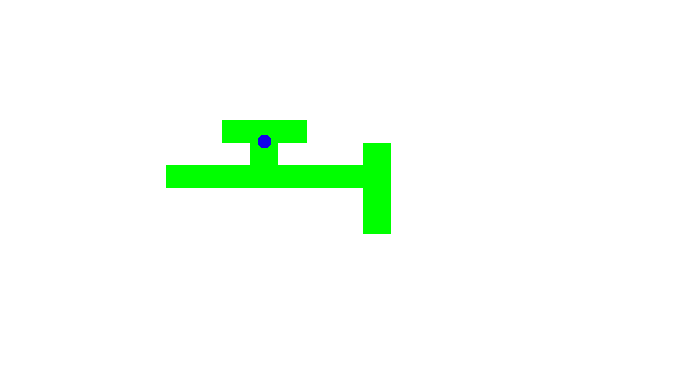
\includegraphics{Images/connected_face.png}}
\caption{\label{fig:Connected Component} Connected Component Containing Origin}
\end{center}
\end{figure}

}




















\frame[allowframebreaks]
{
  \frametitle{Robot Localization Algorithm}


{\bf Input:}\\
Map polygon $P$, the visibility polygon $V$.
\\
{\bf Output:}\\
The robot localizes to its actual position $h \in H$
\\
\begin{algorithmic}[1]
  \STATE Compute the set of hypotheses $H$.
 \WHILE{ $ | H | > 1$ } 
  \STATE Compute the majority-rule map $P_{maj}$
  \STATE {\bf Compute the polygons $G_{ij}$ for each pair of hypotheses, $h_{i}$ and $h_{j}$ }
  \STATE Compute the majority rule map $K_{i}$ of $G_{ij}$'s
  \STATE Find the edges on the boundary of $K_{i}$ which are not on the boundary of $P_{maj}$
  \STATE Draw grids and compute the set of coordinates $Q_{H}$ on these edges.
  \STATE Make instance $I_{P,H}$  of $\frac{1}{2}$ -Group Steiner Problem
  \STATE Solve $I_{P,H}$ to compute a half computing path $C \subset P_{maj}$
  \STATE Half-Localize by tracing $C $ and making observations at coordinates $Q_{H}$
  \STATE Move back to the starting location.
 \ENDWHILE
\end{algorithmic}
}





\frame[allowframebreaks]
{
  \frametitle{Computing the Group Boundaries, $G_{ij}$}

To compute $G_{ij}$ we first compute $F_{ij}$. $F_{ij}$ is the face containing origin in the overlay of polygons $P_{i}$ and $P_{j}$.
The following diagram taken from \cite{key1} demonstrates the notation and the construction.

\begin{figure}[h]
\begin{center}
\scalebox{0.30}{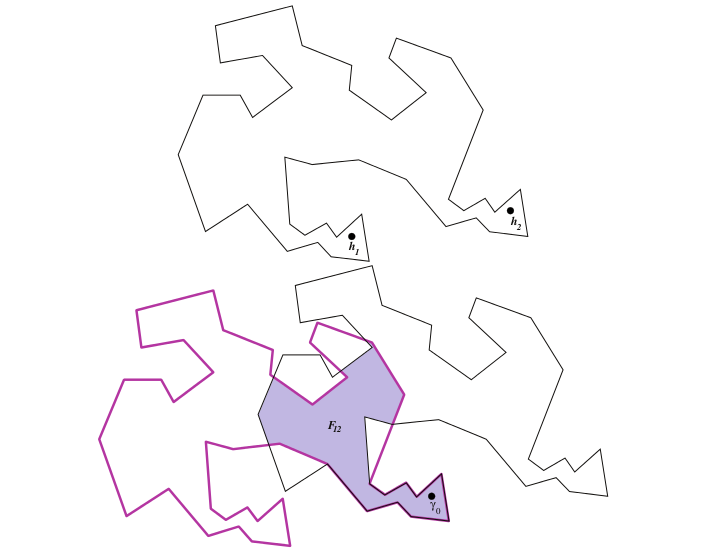
\includegraphics{Images/F12.png}}
\caption{\label{fig:Construction}$F_{12}$}
\end{center}
\end{figure}

}



\frame[allowframebreaks]
{
  \frametitle{Algorithm}

To obtain $G_{ij}$ from $F_{ij}$ we draw visibility polygon of type 1 and type 2 edges and take their lower envelope.
\begin{figure}[h]
\begin{center}
\scalebox{0.40}{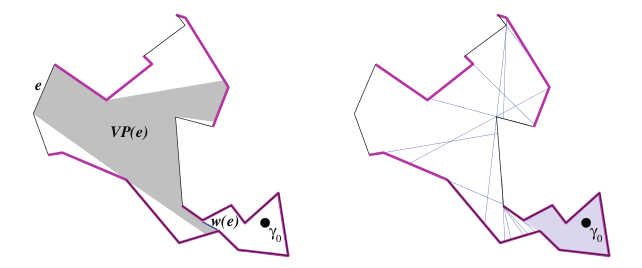
\includegraphics{Images/LowerEnvelope.png}}
\caption{\label{fig:Construction}Lower Envelope}
\end{center}
\end{figure}

Finding the lower envelope is easy using the CGAL's inbuilt Arrangement class. We find the visibility polygon of each edge of type 1
or type 2 and insert it into an arrangement. Later we check the face which contains the point $\gamma_{0}$. This face is nothing else
but $G_{ij}$
The above algorithm is repeated to obtain $G_{i1}$, $G_{i2}$, $G_{i3}$, $G_{i4}$, .... $G_{ik}$.
}


\frame[allowframebreaks]
{
  \frametitle{Examples}

\begin{figure}
\begin{center}
\scalebox{0.40}{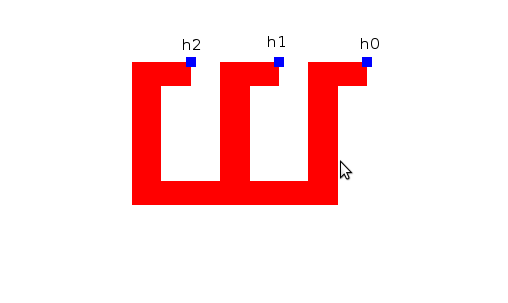
\includegraphics{Images/HypothesisScenario1.png}}
\caption{\label{fig:Construction}Lower Envelope}
\end{center}
\end{figure}


\begin{figure}
\begin{center}
\scalebox{0.40}{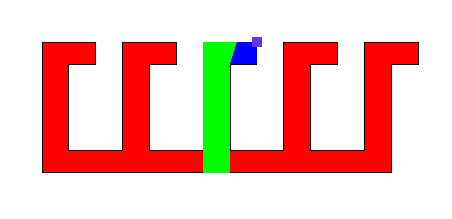
\includegraphics{Images/Map1_G02.png}}
\caption{\label{fig:Construction}Lower Envelope}
\end{center}
\end{figure}


\begin{figure}
\begin{center}
\scalebox{0.60}{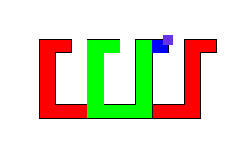
\includegraphics{Images/Map1_G01.png}}
\caption{\label{fig:Construction}Lower Envelope}
\end{center}
\end{figure}


}



\frame[allowframebreaks]
{
  \frametitle{Robot Localization Algorithm}


{\bf Input:}\\
Map polygon $P$, the visibility polygon $V$.
\\
{\bf Output:}\\
The robot localizes to its actual position $h \in H$
\\
\begin{algorithmic}[1]
  \STATE Compute the set of hypotheses $H$.
 \WHILE{ $ | H | > 1$ } 
  \STATE Compute the majority-rule map $P_{maj}$
  \STATE Compute the polygons $G_{ij}$ for each pair of hypotheses, $h_{i}$ and $h_{j}$
  \STATE {\bf Compute the majority rule map $K_{i}$ of $G_{ij}$'s }
  \STATE Find the edges on the boundary of $K_{i}$ which are not on the boundary of $P_{maj}$
  \STATE Draw grids and compute the set of coordinates $Q_{H}$ on these edges.
  \STATE Make instance $I_{P,H}$  of $\frac{1}{2}$ -Group Steiner Problem
  \STATE Solve $I_{P,H}$ to compute a half computing path $C \subset P_{maj}$
  \STATE Half-Localize by tracing $C $ and making observations at coordinates $Q_{H}$
  \STATE Move back to the starting location.
 \ENDWHILE
\end{algorithmic}
}

\frame[allowframebreaks]
{
  \frametitle{Computing the Group Boundaries, $K_{i}$}

To obtain $K_{i}$ we construct the
majority rule map of all $G_{ij}$'s. $K_{i}$ is a region of special interest because of the special following special property. For
proof of it, please refer \cite{key1}
\\
 A robot initially located at $h_{i}$ half localizes if it crosses the boundary of $K_{i}$.
}


\frame[allowframebreaks]
{
  \frametitle{Examples}

For The below map
 the blue region shows $G_{ij}$ and the combined region of blue and green represents $F_{ij}$ in the overlay
arrangement of the polygons $P_i$ and $P_j$.
\begin{figure}
\begin{center}
\scalebox{0.40}{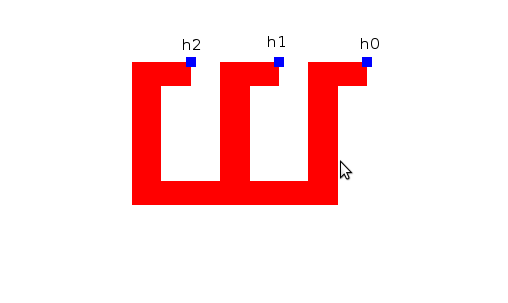
\includegraphics{Images/HypothesisScenario1.png}}
\caption{\label{fig:Construction}Map Polygon with Hypotheses}
\end{center}
\end{figure}

\begin{figure}
\begin{center}
\scalebox{0.40}{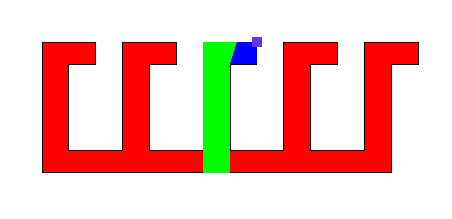
\includegraphics{Images/Map1_G02.png}}
\caption{\label{fig:Construction}$G_{02}$ and $F_{02}$}
\end{center}
\end{figure}

\begin{figure}
\begin{center}
\scalebox{0.40}{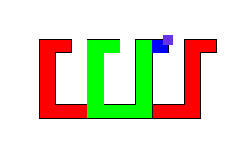
\includegraphics{Images/Map1_G01.png}}
\caption{\label{fig:Construction}$G_{01}$ and $F_{01}$}
\end{center}
\end{figure}

\begin{figure}
\begin{center}
\scalebox{0.50}{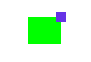
\includegraphics{Images/Ki.png}}
\caption{\label{fig:Construction} $K_{1}$}
\end{center}
\end{figure}

}




\frame[allowframebreaks]
{
  \frametitle{Robot Localization Algorithm}


{\bf Input:}\\
Map polygon $P$, the visibility polygon $V$.
\\
{\bf Output:}\\
The robot localizes to its actual position $h \in H$
\\
\begin{algorithmic}[1]
  \STATE Compute the set of hypotheses $H$.
 \WHILE{ $ | H | > 1$ } 
  \STATE Compute the majority-rule map $P_{maj}$
  \STATE Compute the polygons $G_{ij}$ for each pair of hypotheses, $h_{i}$ and $h_{j}$
  \STATE Compute the majority rule map $K_{i}$ of $G_{ij}$'s
  \STATE {\bf Find the edges on the boundary of $K_{i}$ which are not on the boundary of $P_{maj}$ }
  \STATE {\bf Draw grids and compute the set of coordinates $Q_{H}$ on these edges. }
  \STATE Make instance $I_{P,H}$  of $\frac{1}{2}$ -Group Steiner Problem
  \STATE Solve $I_{P,H}$ to compute a half computing path $C \subset P_{maj}$
  \STATE Half-Localize by tracing $C $ and making observations at coordinates $Q_{H}$
  \STATE Move back to the starting location.
 \ENDWHILE
\end{algorithmic}
}

\frame
{
  \frametitle{Computing Reference Points $(Q_{H})$}

\begin{definition}
 {\bf Reference Points:} are the discrete set of points on the edges of $\partial K_{i} \cap \partial G_{i}$  which are used to determine the
  half localization path of robot [see \cite{key5}].   
\end{definition}

\begin{definition}
 {\bf Half Localization Path:} is the path travelling along which the robot can eliminate half of the hypotheses by making
 observations at the reference points.
\end{definition}
}



\frame
{
  \frametitle{Examples}
\begin{figure}[h]
\begin{center}
\scalebox{0.25}{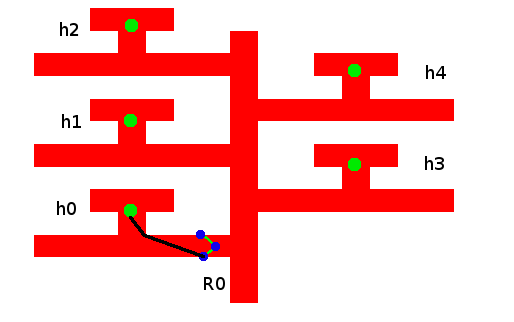
\includegraphics{Images/reference.png}}
\caption{\label{fig:Reference Points}Reference Points in blue color and hypotheses in green color}
\end{center}
\end{figure}

The reference points shown in the figure are for the hypothesis $h_0$. The robot on following the path from $h_0$ to $R_0$ 
can differentiate between hypotheses $\{h_0,h_1,h_2\}$ and $\{h_3, h_4\}$ based on its observation at $R_0$. The path shown in black is the half computing path.
}




\frame[allowframebreaks]
{
  \frametitle{Algorithm}

\begin{enumerate}
 \item For every $i$ find those edges in $K_i$ which are not part of the boundary of majority map. These are important edges on which
we will find out reference points. Let $L_i$ contains all these edges for a particular $i$.
 \item  Calculate $r_0$(geodesic) radius of the smallest geodesic disk centered on $\gamma_{0}$ that intersects at least half of $L_{i}'s$.
\begin{enumerate}
 \item For all $i$ calculate the minimum distance between $\gamma_{0}$ and any of the line segments of $L_i$.
 \item Take the median of all the distances calculated above as the geodesic radius$(r_0)$. 
\end{enumerate}
 \item Let $k$ be the number of hypotheses and $R$ be a sequence of radii $r_0,2*r_0,4*r_0 \dots , 2^{\lceil \log_{2}k \rceil}$.
 \item For every hypothesis $i$ perform the following steps
\begin{enumerate}
 \item Place each line segment $\sigma$ in $L_i$ on an axis aligned square centered at $\gamma_{0}$ of side length $2*2^{j}*r_0$ (where $j$ from $(0..\lceil \log_{2}k \rceil)$)
 \item Decompose the square into $kxk$ grid using $k-1$ horizontal and vertical lines.
 \item Calculate the intersection of the line segment with the grid line. These intersection points are the reference points. Also include 
 end points of the line segment(even if they do not lie on grid) in the set of reference points.  
\end{enumerate}

\end{enumerate}
}



\frame[allowframebreaks]
{
  \frametitle{Examples}

\begin{figure}
\begin{center}
\scalebox{0.30}{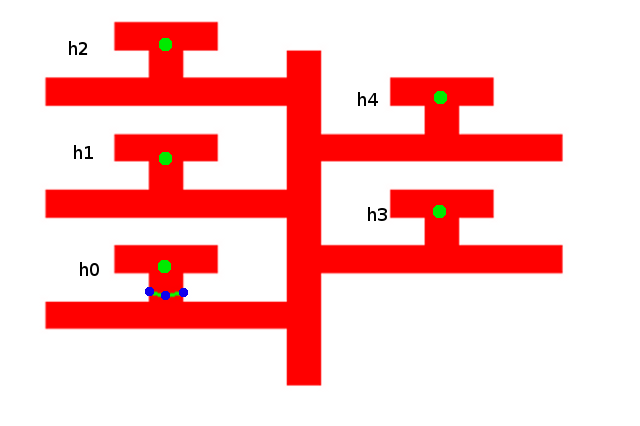
\includegraphics{Images/reference1.png}}
\caption{\label{fig:Construction}Reference Points in blue color and hypotheses in green color}
\end{center}
\end{figure}

\begin{figure}
\begin{center}
\scalebox{0.30}{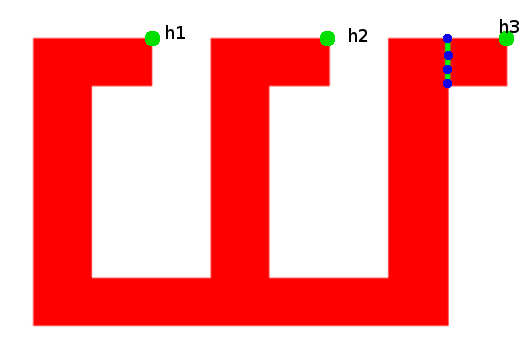
\includegraphics{Images/reference2.png}}
\caption{\label{fig:Construction}Reference Points in blue color and hypotheses in green color}
\end{center}
\end{figure}
}




\frame[allowframebreaks]
{
  \frametitle{Bibliography}

\bibliographystyle{plainnat}
%\bibliographystyle{Classes/IITRPRbiblio}
\renewcommand{\bibname}{References} % changes default name Bibliography to References
\bibliography{References/references} % References file

}


\end{document}
